\documentclass[external]{20120615_deliverable_template_ukob}

\usepackage{xspace}
\usepackage{amsmath,amsthm,amssymb,url,color}
\theoremstyle{definition}
\newtheorem{example}{Example}
\usepackage{xcolor}
\usepackage{color, colortbl}
\usepackage{subfigure}
%\usepackage{showkeys}

\newcommand{\todo}[2]{\textcolor{magenta}{#1: #2}}

\LGtitle{\LiveGovThirtyTitleFonts \textbf{D1.2 - Mobile Sensor App with Mining Functionality} }
%\LGnumber{WP.NR} % e.g 6.7 no letters D or ID

\LGnumber{1.2}

\LGwp{WP1 - Reality Sensing and Mining}

\LGdissemination{PU - Public}

\LGcontractdate{Month 27, March 2014}

\LGactualdate{Month 26, February 2014}

\LGtask{T1.1, T1.2, T1.3}

\LGtype{Prototype}

%\LGnature{$<$ Report $|$ Prototype $|$ Demonstrator $|$ Other $>$}

%\LGapproved % activate only if approved
\LGdraft

\LGversion{Alpha 0.4}
%\LGstaffmonths{Resources spent on the deliverable}

%\LGdistribution{WP leaders, PMB members, European Commission}

%\LGkeywords{}


%\LGabstract{Put abstract here (separate paragraphs using
%{\tt\char92 par}.)}
\LGabstract{ 

\todo{HH}{Add abstract}

%  This deliverable describes the mobile sensor mining component.
%  Along with this document we supply the source code of the
%  components, documentation (javadoc), and pre-compiled packages for
%  direct installation and testing on mobile devices.  

}

%\LGhistory{01}{2011-10-01}{First draft}{Yiannis Kompatsiaris}
%\LGhistory{02}{2011-10-02}{Modifications}{Sotiris Diplaris}
%\LGhistory{03}{2011-10-03}{Further Modifications \& Corrections}{Sotiris Diplaris}
%\LGhistory{04}{2011-10-05}{Further Modifications \& Corrections}{Sotiris Diplaris}


%------------------------ macro for change portrait to landscape
\usepackage{calc,graphicx,pdflscape,eso-pic} % needed for printing
                                             % headers and footers
\newlength\landscapewidth
\newlength\landscapeheight
\newcommand\landscapepagestyle{ % command which prepare page
                                % for landscape printing,
                                % change to landscape is
                                % achieved by pdflscape
\clearpage \thispagestyle{empty}
\setlength\landscapewidth{247mm}
\setlength\landscapeheight{161mm}
\AddToShipoutPicture*{\AtPageCenter{ % this make "layer" for
                                     % printing the header and footer
\rotatebox[origin=c]{90}{
\hspace*{-2em} % for adjusting position of
               % header and footer
\parbox{\landscapewidth}{\vskip-.57\landscapeheight
%\centerline{\WEKNOWIT \hfill \textbf{\Large \bf{IDx.x - V0} \normalsize }} %header text for Internal Deliverables
                                                                         % notation: IDx.x V{LGversion}
\centerline{\LiveGovLogo \hfill \textbf{\Large \bf{Dx.x - V0} \normalsize }} %header text for External Deliverables
                                                                        % notation: Dx.x V{LGversion}
\vspace{-5pt} \rule{\landscapewidth}{0.4pt} \\
\rule{0pt}{\landscapeheight} \\
%\rule{\landscapewidth}{0.4pt} \\
\centerline{Page \thepage\ }  % footer text
} } } } }

%--------------------------------------------------------------------------------------------------------------%
\usepackage{appendix}
\pretolerance=10000 % prevent overflow lines for $math$ elements

\begin{document}

% add a \LGaddhistory{version}{date}{reason}{revised by} for each new
% version
\begin{LGhistory}
\LGaddhistory{0.1}{2013-10-14}{Outline}{Heinrich Hartmann}
\LGaddhistory{0.2}{2014-01-06}{Added section on topic modeling}{Christoph Kling}
\LGaddhistory{0.3}{2014-01-07}{Revised Outline}{Heinrich Hartmann}
\LGaddhistory{0.4}{2014-01-07}{Alpha Version}{Heinrich Hartmann}

\end{LGhistory}


\newcommand{\LGaddauthorNoPhone}[3]{\hline  #1 &  #2 & %
   \parbox{3em}{E-mail:} \small #3 \\
}

% add a
% \LGaddauthor{Partner}{Name}{Telephone}{Fax}{Email} for each author
\begin{LGauthors}

\LGaddauthor{UKob}{Heinrich Hartmann}{+49 261 287 2759}%
{+49 261 287 100 2759}{\small hartmann@uni-koblenz.de}

\LGaddauthor{UKob}{Christoph Schaefer}{+49 261 287 2786 }%
{+49 261 287 100 2786}{\small chrisschaefer@uni-koblenz.de}

\LGaddauthor{UKob}{Christoph Kling}{+49 261 287 2702}%
{+49 261 287 100 2702}{\small ckling@uni-koblenz.de}

\LGaddauthor{UKob}{Daniel Janke}{+49 261 287 2747}%
{+49 261 287 100 2747}{\small danijank@uni-koblenz.de}

\LGaddauthorNoPhone{MTS}{Laura Niittyl\"a}%
{\small Laura.Niittyla@mattersoft.fi}

\end{LGauthors}



\begin{LGExecutiveSummary}
  \vspace{10pt} 

\todo{HH}{Add Summary}

\end{LGExecutiveSummary}


% add a \LGaddabbreviation{ABBR}{Explanation} for each abbreviation
\begin{LGAbbreviations}
%\LGaddabbreviation{LG}{Live+Gov}

\LGaddabbreviation{\textbf{API}}
{Application Programming Interface}

\LGaddabbreviation{\textbf{GPS}}
{Global Positioning System}

\LGaddabbreviation{\textbf{GSM}}
{Global System for Mobile Communications}

\LGaddabbreviation{\textbf{HTML}}
{HyperText Markup Language}

\LGaddabbreviation{\textbf{HTTP}}
{Hypertext Transfer Protocol}

\LGaddabbreviation{\textbf{JSON}}
{JavaScript Object Notation}

\LGaddabbreviation{\textbf{REST}}
{Representational State Transfer}

\LGaddabbreviation{\textbf{SVM}}
{Support Vector Machine}

\LGaddabbreviation{\textbf{URL}}
{Uniform Resource Locator}

\LGaddabbreviation{\textbf{UUID}}
{Universal Unique Device Identifier}

\LGaddabbreviation{\textbf{WP}}
{Work Package}

\LGaddabbreviation{\textbf{WIFI}}
{Wireless Fidelity (IEEE 802.11), WLAN}

\LGaddabbreviation{\textbf{WLAN}}
{Wireless Local Area Network}

\LGaddabbreviation{\textbf{XML}}
{Extensible Markup Language}

\LGaddabbreviation{~\\}
{~~~}

\end{LGAbbreviations}

% add a \LGaddterm{Term}{Explanation} for each entry of the glossary
%\begin{LGGlossary}
%\LGaddterm{Term}{Definition text here}
%\LGaddterm{Term2}{Definition text here}
%\end{LGGlossary}

\setcounter{tocdepth}{1}

% add this for a table of contents
\LGTOC

\newpage

\chapter{Introduction}
\label{chap:Introduction}
\todo{HH}{Write Introduction}

\section{Description of Deliverable D1.2}
Sensor Data App with Mining Functionality: This deliverable will provide the
extended version of the data capturing prototype for mobile devices, with
implemented reality mining methods and optimized communication interfaces for
result transmissions to the application server.

\section{Task Descriptions}
\begin{itemize}
\item[T1.1] {\bf Sensor and user input data capturing} \\
  This task will first define a taxonomy of classifications that are useful to
  determine for contextualization of citizens’ uploads including activity
  profiles (e.g. walking, cycling, riding train, riding bus,...) and coarse
  issue classifications (street, people, traffic,...). Research investigations
  will determine how these categories can be captured and classified
  economically using limited battery power (e.g. trading off between power
  draining sensors like GPS or audio by less expensive ones like accelerator
  monitoring) and limited bandwidth to the Live+Gov backbone server. The task
  also comprises the contextualized capturing of citizen text, deictic or voice
  input while accounting for limitations of mobile hardware and communication
  channels.
\item[T1.2] {\bf Smartphone based reality mining} \\
  In this task we will develop memory and energy aware mining mechanisms for
  exploiting data collected in T1.1 for various kinds of initial processing on
  mobile devices - including classification, filtering, abstraction, and
  personalization. The key concern of our development will be on wide usability
  of reality mining methods and their flexible applicability for dynamic user
  contextualization in project scenarios.
\item[T1.3] {\bf Server based reality mining} \\
  Based on limited analysis of data in T1.2 and based on citizens’ preferences
  and explicit consent, (possibly) abstracted sensor data will be uploaded to
  the Live+Gov backbone where further mining will occur. We will develop mining
  methods which are needed for the application, but cannot be run on individual
  smartphones (e.g.  because input from multiple users is needed). In
  particular, this will comprise the detection of common patterns delivered from
  many citizens, but also outlier detection and treatment, which is required to
  discover spoofing or important emergencies. The methods resulting from this
  task will be particularly relevant for supporting augmented reality
  applications (WP3) and contextualization of data mining results in eGovernance
  scenarios in line with policy models (WP2).
\end{itemize}


\clearpage
\chapter{Sensor Collection Service}
\todo{HH}{Add content}

Explain the improvements of the sensor collection service since D1.1

In particular cover the topics:
\begin{enumerate}
\item Improved Architecture Description
\item Inspection Front End
\item New Sensor Transfer File Format
\item New Streaming API
\item Integration Loging and Heartbeating into Upload Servlet
\item Data Collection event in Koblenz
\end{enumerate}

\chapter{Reality Mining Methods}

\section{Human Activity Recognition}
\todo{HH}{Add content.}

\subsection{Related Work}
Explain common approaches to human activity recognition, evaluation
methods and resulted quality.

\subsection{Component Description}
Explain our own implementation:

\begin{enumerate}
\item Architecture Description (Class diagrams, DB Schemes)
\item Decision Tree classifier
\item PCA-SVM based classifier
\end{enumerate}

\subsubsection{SVM based classifier}

A popular algorithm to train a binary classification model for mapping features to activities is the Support Vector Machines (SVMs). SVMs are known for their ability in smoothly generalizing and coping efficiently with high-dimensionality pattern recognition problems. They define a hypothesis space that includes all the possible linear separations of the data (see Fig.~\ref{fig:svm_hypothesisSpace}) and they choose the one that maximizes the margin between the two classes (Fig.~\ref{fig:svm_margin}). 



\begin{figure}[h]
\centering
  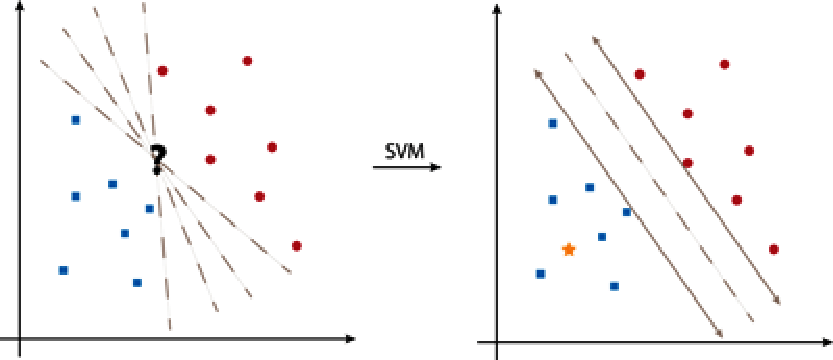
\includegraphics[width=0.4\textwidth]{img/svms/Svms_hypothesisSpace.pdf}
  \caption{Left: Hypothesis space including all linear separations. Right: The selected hypothesis maximizes the margin.}
  \label{fig:svm_hypothesisSpace}
\end{figure}


\begin{figure}[h]
\centering
  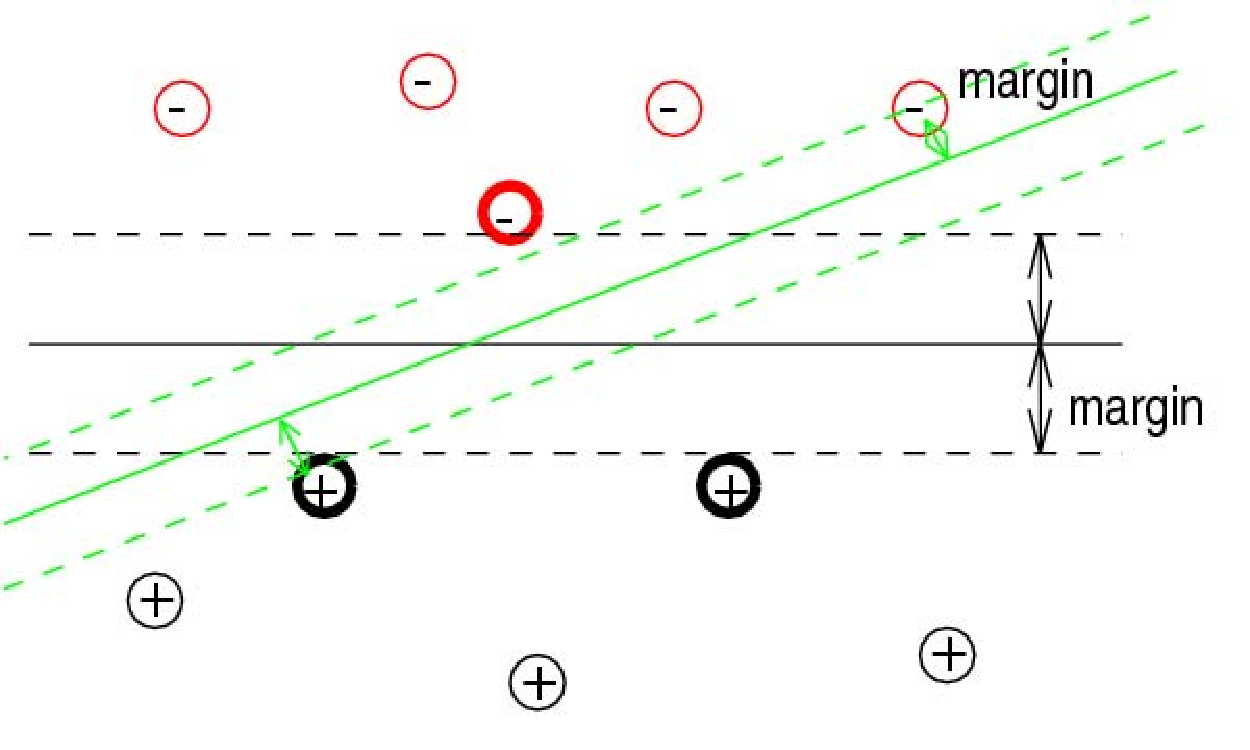
\includegraphics[width=0.5\textwidth]{img/svms/Svm_Maxmargin.pdf}
  \caption{Maximization of the margin}
  \label{fig:svm_margin}
\end{figure}

\noindent The hyperplane that optimally separates the positive and the negative class (i.e. maximizes the hyperplane) can be described by $\mathbf{w\cdot x + b = 0}$, where $\mathbf{w}$ is normal to the hyperplane and $\frac{b}{\parallel\mathbf{w}\parallel}$ is the perpendicular distance from the hyperplane to the origin (Fig.~\ref{fig:svm_wb}). The optimal hyperplane can be obtained by solving the following Quadratic Programming optimization problem:

\begin{equation}\label{Eq:svmQP0}
\min \frac{1}{2}\parallel\mathbf{w}\parallel \quad \text{s.t.} \quad y_i(\mathbf{w}\cdot x_i + b) -1 \ge 0 \quad \forall i
\end{equation}

In order to relax the constraints of Eq.~\ref{Eq:svmQP0} and allow for some misclassified points a slack variable $\xi_i, i=1,\ldots,L$ is introduced which modifies Eq.~\ref{Eq:svmQP0} into:

\begin{equation}\label{Eq:svmQPxi}
\min \frac{1}{2}\parallel\mathbf{w}\parallel + C\sum_{i=1}^{L}\xi_i \quad \text{s.t.} \quad y_i(\mathbf{w}\cdot x_i + b) -1 +\xi_i \ge 0 \quad \forall i
\end{equation}

\noindent where the parameter $C$ controls the trade-off between the slack variable penalty and the size of the margin. In the testing phase, in order to classify an unseen example $x_t$, its distance to the hyperplane is calculated using the formula $\mathbf{w}\cdot x_t + b$. This distance 


\begin{figure}[h]
\centering
  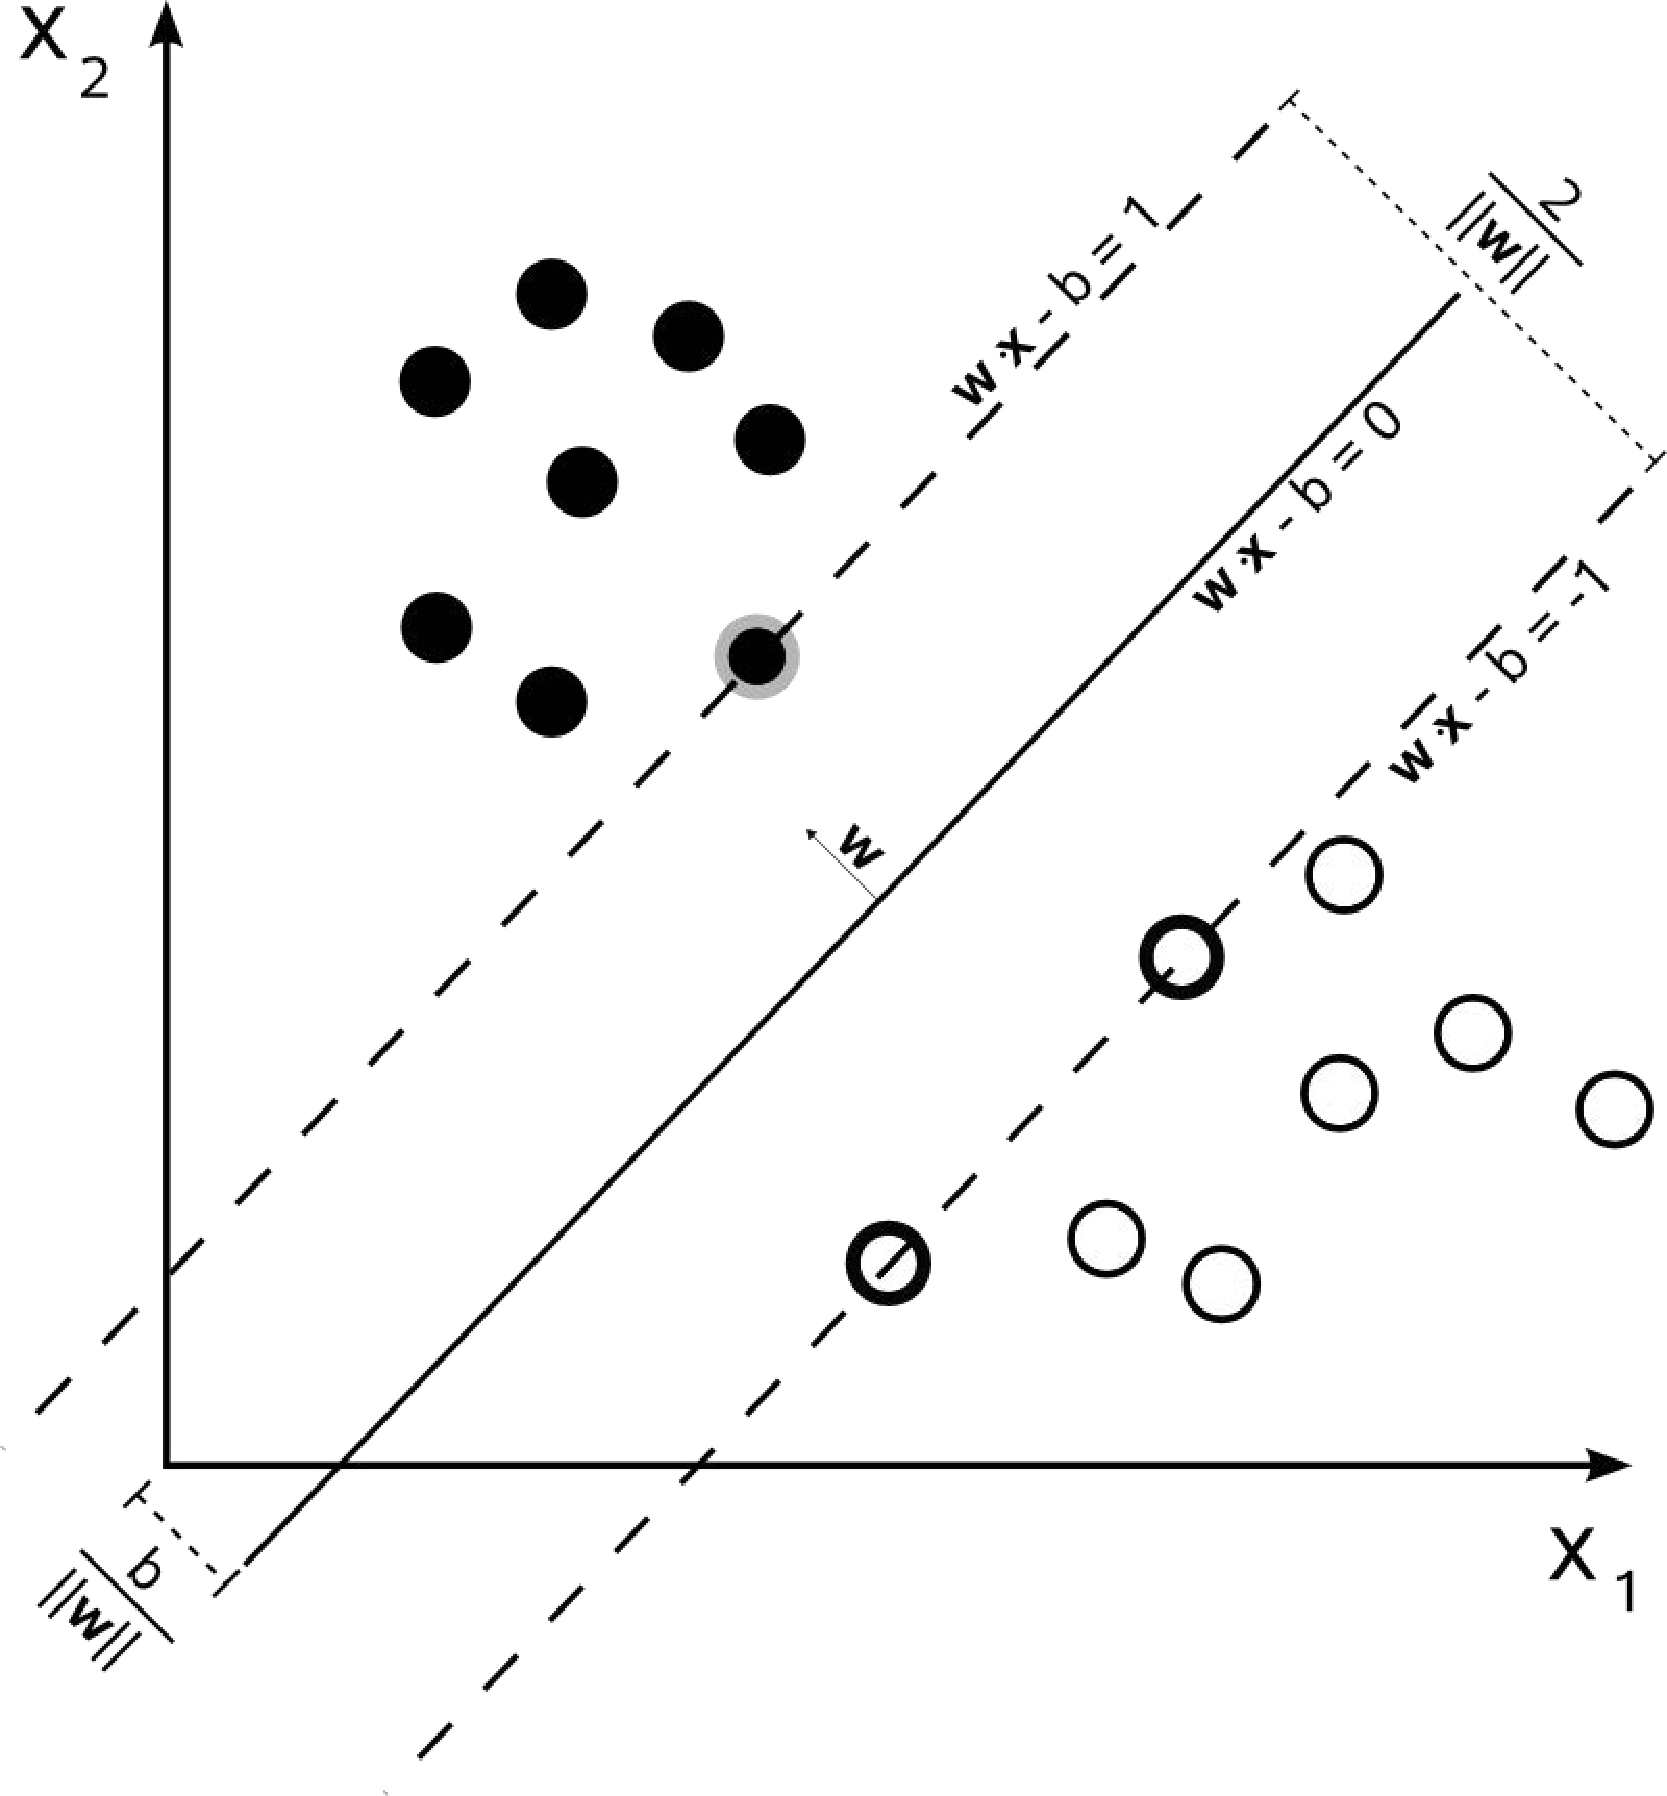
\includegraphics[width=0.4\textwidth]{img/svms/Svms_wb.pdf}
  \caption{Maximization of the margin}
  \label{fig:svm_wb}
\end{figure}

An SVM model is trained on the previously extracted features in order to learn the properties that define the examined activity. The models are trained using the one versus all (OVA) technique, i.e. all positive examples of the specific activity versus all negative examples. The classification model learns the hyperplane that best separates the space of the positive and negative samples, by maximizing the margin between the two classes. Applying the kernel trick, we can map the features to a higher dimension and at the same time consider the cases where the classes are not linearly separable. For example, in the case of a linear kernel the model considers linear separation of the data, while in the case of an RBF kernel the hyperplane is a hypersphere. For any kernel $K(x,y)$, the classification model can be represented by a vector $\textbf{w}$ (i.e. the model parameters), a bias scalar $b$ and the support vectors $\mathbf{SV}_j, j=1,\ldots,N_{SV}$. For an activity $a$ and a test window $i$, which corresponds to a feature vector $\textbf{f}_i$, a confidence score is extracted by computing its distance to the hyperplane of the model for the activity $a$:

\begin{equation}\label{Eq:SVMdecision}
  confidence(i,a) = \mathbf{w}_a*\sum_{j=1}^{N_{SV}}{K(\mathbf{SV}_j,\mathbf{f}_i)}+b_a
\end{equation}

The distance of a vector from the hyperplane indicates our confidence that during the examined window, the user performs the specified activity. High positive values of this score increase our confidence that this window belongs to the positive class while high negative values provide strong confidence that the performed activity is not the examined one. 

%The fact that each model can be represented by a single vector and a scalar and that the testing process is essentially a vector multiplication, renders SVMs the best solution for a real time classification framework. This allows for storing the information about all the models in the phone memory, while testing is computationally very efficient, making it possible for the image classification algorithm to run entirely on a mobile phone.

\subsection{Cross-Platform Strategy}
Explain problems with Titanium framework.

Android component runs on Blackberry. 

Implement HAR as SAAS. Write client app for iOS.

\subsection{Evaluation}
Comparison of our classifier with literature on the basis of external
data sets.

\section{Service Line Detection}

One part of the user contextualization is the service line detection. The aim of this component is to recognize if a citizen uses public transport within the HSL area in Helsinki. If such a usage is detected, the right service line id with its direction and the further itinerary will be determined. Based on this information it is possible to solve higher level tasks like traffic jam detection, connecting train recommendation, or network utilization analysis.

The service line detection is implemented as a server side mining component which provides a REST API for answering user queries in real time. For long term evaluations all API calls are recorded and send to the L+G Service Center on a daily bases. Due to the seamless integration into the L+G ecosystem, where each user gets an universal unique id, all received tracks are personalized and can be combined with additional information coming from other components. In a later analysis, the service line detection results can be augmented with the low level human activity recognition data of the same user to gain a better insight into the users behavior.

\begin{figure}[ht]
\centering
\subfigure[]{
  \frame{\includegraphics[width=0.3\textwidth,natwidth=556.19,natheight=432]{img/SLD/track.pdf}}
  \label{fig:track}
  \setcounter{subfigure}{1}
} 
\subfigure[]{
  \frame{\includegraphics[width=0.3\textwidth,natwidth=556.19,natheight=432]{img/SLD/realtime.pdf}}
  \label{fig:realtime}
  \setcounter{subfigure}{2}
}
\subfigure[]{
  \frame{\includegraphics[width=0.3\textwidth,natwidth=556.19,natheight=432]{img/SLD/static.pdf}}
  \label{fig:static}
  \setcounter{subfigure}{3}
}
\subfigure[]{
  \frame{\includegraphics[width=0.3\textwidth,natwidth=556.19,natheight=432]{img/SLD/interpolatedCoords.pdf}}
  \label{fig:interpolatedCoords}
  \setcounter{subfigure}{4}
}
\subfigure[]{
  \frame{\includegraphics[width=0.3\textwidth,natwidth=556.19,natheight=432]{img/SLD/interpolatedCoordsWithTimes.pdf}}
  \label{fig:interpolatedCoordsWithTimes}
  \setcounter{subfigure}{5}
} 
\subfigure[]{
  \frame{\includegraphics[width=0.3\textwidth,natwidth=556.19,natheight=432]{img/SLD/combined.pdf}}
  \label{fig:combined}
  \setcounter{subfigure}{6}
}
\caption{
The various input data for the HSL service line detection.
}
\label{fig:SLD}
\end{figure}

Assigning a trajectory to a specific service line requires the access to suitable background knowledge. In the Helsinki case it is two fold:
First of all, the system is fed with all HSL public transportation schedules and associated geographic information of stops and travel paths. By means of this dataset the theoretical position of every vehicle at any point in time can be calculated. A drawback of only including static time tables is that actual schedule deviations stay disregarded. This gap is closed by the HSL Live API, which is the second data source the service line detection relies on. With this API, the actual positions of some vehicles can be determined. Especially trams are tracked in realtime and can be accessed via this interface.  Unfortunately, the vast majority of vehicles, such as buses, have not yet been integrated. Lacking a complete realtime coverage is why still some uncertainty remains in the overall system. Therefore, the main challenge is to combine both kinds of data to archive the best possible performance.

Just as the background data, the classification algorithm is also two-stage. Given an user trajectory containing a small set of GPS coordinates with timestamps (Figure~\ref{fig:track}), in a first step the algorithm checks if the latest given timestamp is near the actual time. If so, the HSL Live API is called in order to find all vehicles which are currently around the user (Figure~\ref{fig:realtime}). Service lines found below a certain distance to the user are scored with a high probability to be the true line belonging to the given track.

In a second step, each coordinate of the given track is compared to the static route data (Figure~\ref{fig:static}) obtained from the time tables and paths.
It should be noted that the public transportation schedules only contain exact arrival times for each stop, but don't provide any time data for the pathes between them. Since this data is too sparse to perform reliable service line detection on it, all paths are rasterized evenly (Figure~\ref{fig:interpolatedCoords}) and the corresponding time for each intermediate part is interpolated (Figure~\ref{fig:interpolatedCoordsWithTimes}). This ensures that no route section falls through the cracks when executing a simple distance query in time and space. Figure~\ref{fig:combined} shows the combined view of all data used for the HSL service line detection.

The result of the algorithm is the one service line which has the highest probability due to the Live API and/or the smallest distance to the given set of coordinates. During a testing phase, the optimal values of all involved parameters like distance thresholds, time and space raster sizes, and the individual scoring weights have to be learned. As one outcome of the Helsinki field trial, we expect to find a good heuristic how to setup the various ingredients of the algorithm.

\subsection{Implementation details}
As a starting point, HSL provided us with all static service line data like arrival times, stop positions, route meta data, and path files in the well known General Transit Feed Specification (GTFS)\footnote{\url{https://developers.google.com/transit/gtfs/}} format. The original data set had a size of 400 MB and was imported into a PostgreSQL database. All paths and stop positions were stored as native geospatial values using PostGIS, a spatial database extender for PostgreSQL. After the import, we found 587 distinct routes, 7534 stops, and a total number of 206,153 trips in the database. In general, a service line like the bus 934 from Myyrm\"{a}ki to Luhtaanm\"{a}ki, has two directions, travels along its route path and stops at its stops. If a service line runs every ten minutes, each trip has its own trip id and is uniquely identifiable.

While these data are too sparse for distance queries, we interpolate the possible positions of a vehicle along its path to ensure that the distance between two consecutive trip positions is always smaller than ten meter. On the one hand, this simplifies a query like "find all trips in a distance of 20 meters around the user which arrive in plus minus one minute from now" a lot. On the other hand, the interpolation and denormalization inflates the data. Resulting in 324,440,457 trip positions annotated with arrival time and trip id, we enlarged the original data to a size of 38 GB.

This size leads the PostGIS index to its limit and prevents response times below 30 seconds for a service line detection query. Therefore, all data was partitionated horizontally in time dimension. The reason is, that all time tables repeat itself every 7 days and an usual query covers only a very small period of time at a specific weekday. Against this background, we divided the data into 24 parts for every day, which results in 7 times 24 subtables in the database. Finally, this setting archives average response times of less than one second for a whole service line detection query, containing of up to 200 single distance queries.


\subsection{Evaluation}
How did we test the quality of the classifier.

\section{Traffic Jam Detection}
\todo{MTS}{Add content.}

\subsection{Related Work}
Explain common approaches to Traffic Jam detection or related problems.

\subsection{Component Description}
Explain implementation. 

\subsection{Evaluation}
How was the quality of the jam detection classifier assessed?

\section{Distributed Geo-Matching}
\todo{DJ}{Add content.}
\input{sections/DistributedGeoMatching}

\section{Geographic Topic Analysis}
\input{sections/TopicModels}

\bibliography{D1-2}

\end{document}
